\chapter{History}
	\index{history}
    \label{chap:history}
	I had the pleasure of being invited to present at an Art Gallery Exhibit in \index{Goombungee}Goombungee, \textit{Gumna No Sheila}, in \index{Goombungee}Goombungee in the month of November, 2014.\\
    	
    The show revolved around "things men do in their sheds". Ranging from steam machinery, wood sculptures, motor bikes, kites... and our \index{robotics}robotics.\\
	
	\section{BaralabaBob}
    	\index{BaralabaBob}
		BaralabaBob (the \index{hexapod}hexapod, talked about in the \index{robotics}\hyperref[chap:Robotics]{Roobtics} chapter had been ordered several months previously, and arrived just in time for me to prepare it for the show. I spent the month of October preparing, but specifically from the 12th-18th of October, in which time I assembled and wrote the code to control \index{BaralabaBob}BaralabaBob.\\
		
		This show is significant because in preparation for it, I was essentially preparing the building blocks for RoboCup. A lot of the code I wrote for \index{Goombungee}Goombungee I use today.\\
		
		The \index{hexapod}hexapod had to be left, without my human presence, in \index{Goombungee}Goombungee for 30 days. To that point I had never developed a \index{system}system that had to operate for more than a few minutes - this presented its own challenges in me trying to design it as \index{reliably}\index{reliability}reliably as possible.\\
		
		\centerline{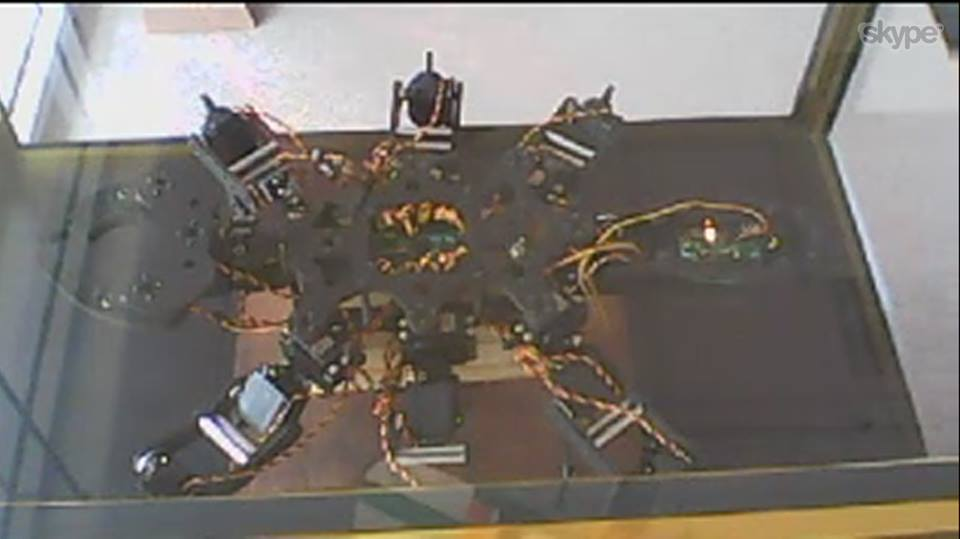
\includegraphics[width=0.75\linewidth]{images/goombungee_skype}}
		\vspace{5pt}
		\centerline{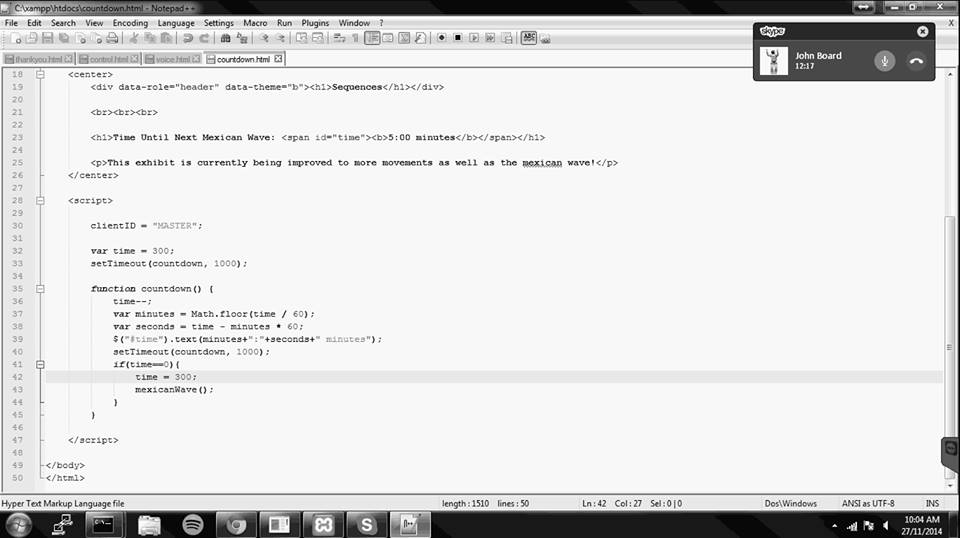
\includegraphics[width=0.75\linewidth]{images/goombungee_js}}
		\vspace{5pt}
		\centerline{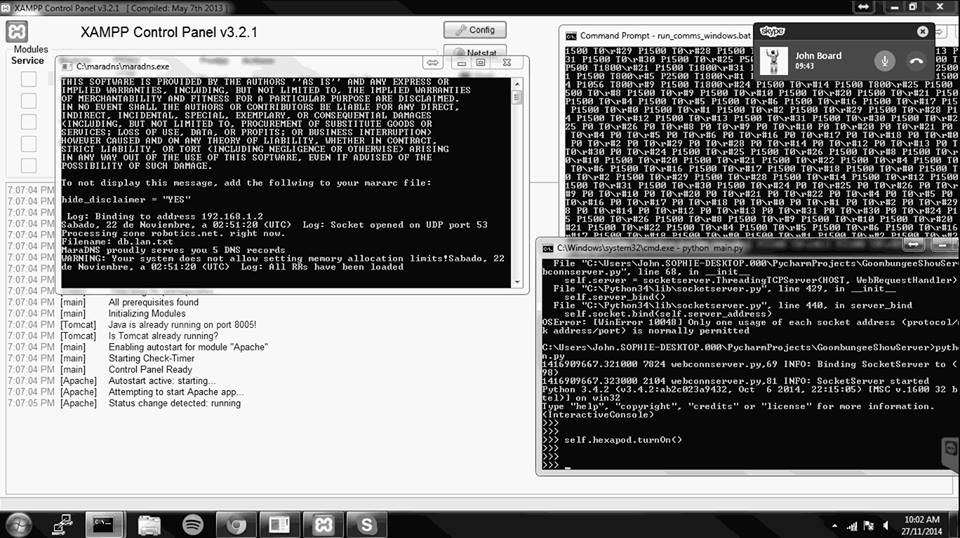
\includegraphics[width=0.75\linewidth]{images/goombungee_teamviewer}}
		\pagebreak
		
		Although the system I created was fairly \index{reliable}reliable, I did have a few computer problems which I had to sort out \index{remotely}remotely, by means of instructed a human over telephone how to reboot my systems, and connect me to the internet. These were quite \index{challenges}challenging, but all challenges were overcome.\\
		
		The result of these efforts meant I created a very \index{reliable}reliable and well rounded \index{codebase}codebase right from the start. Originally the code was designed to run on an external Windows 7 desktop, however I was able to easily port the \index{python}python code to operate on the now \index{Raspberry Pi}Raspberry Pi.\\
		
	\section{Beaker}
		As well as having an exhibit set up, I visited \index{Goombungee}Goombungee for a weekend to give talks, and personally present the robot. During that time I set up "shop" in the attached \index{library}Library. In the library I had several interactive exhibits which people could visit and play with. I also presented a few talks, aided with a \index{PowerPoint}PowerPoint, to visitors.\\
		
		One of the \index{interactive}interactive robots was \index{Beaker}\hyperref[sec:Beaker]{Beaker}, a plywood \index{robot}robot with electric-car-seat \index{motors} (see it's section in the Robots chapter for more information).\\
		
		\centerline{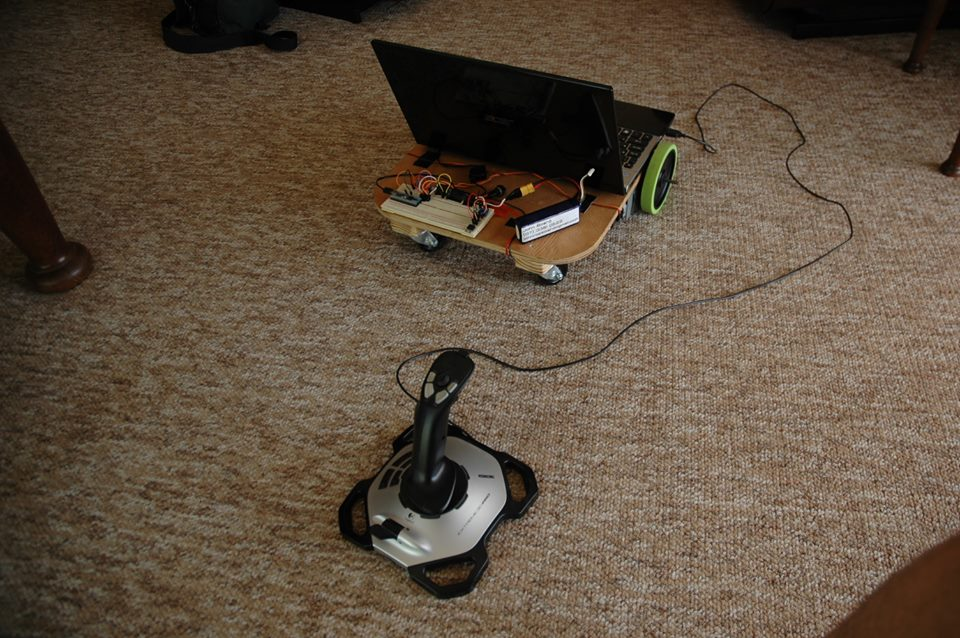
\includegraphics[width=0.75\linewidth]{images/beaker_joystick}}
		
		\index{Beaker}\hyperref[sec:Beaker]{Beaker} was mounted with an Apple MacBook Air, which was connected to a private wireless network I maintained in the Library. Then my laptop, with my joystick connected, would send messages from the laptop over wireless to the MacBook which was connected via serial to a Propeller Chip which would receive the signals, and then send them on to two HB-25 motor drivers.\\
		
		People could control \index{Beaker}\hyperref[sec:Beaker]{Beaker} using the \index{joystick}. I had also \index{prototyped}prototyped a system which would use the skeleton tracking capabilities of the \index{Microsoft}Microsoft \index{Kinect}Kinect to control \index{Beaker}\hyperref[sec:Beaker]{Beaker}. Although people could control it using hand gestures, I noted that they generally opted to go for the tactile \index{joystick}.\\
	
		\centerline{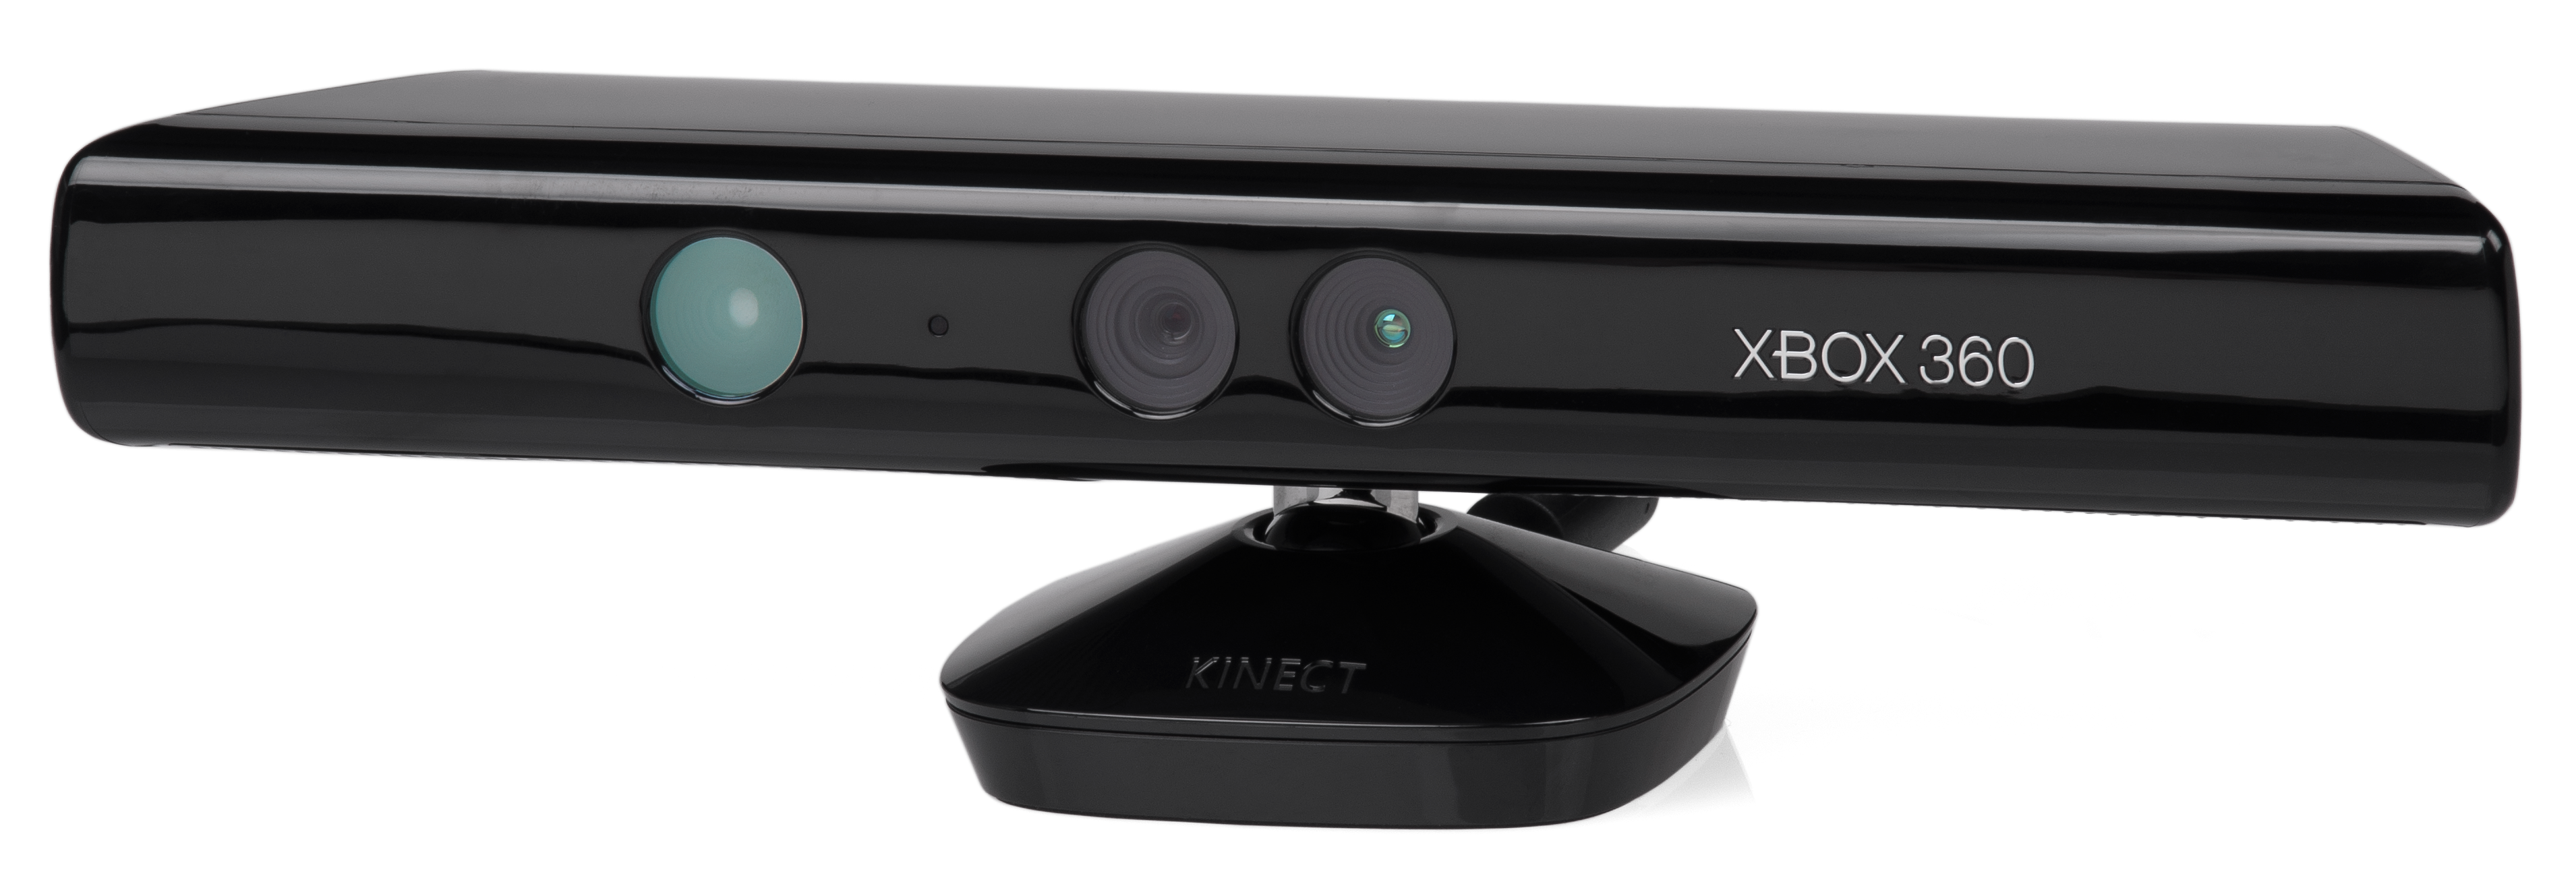
\includegraphics[width=0.75\linewidth]{images/kinect}}
		
	\section{Conclusion}
		\index{Goombungee}Goombungee was a good time, in which I \index{learned} many valuable skills such as designing long term and \index{reliable}reliable systems, improved my public speaking, improved tech support communication over the telephone,  and learned a bit more about how humans interact with robots - amongst many things.\\
		
		\index{Goombungee}Goombungee also provided a solid code base from which I could build the later systems for RoboCup from.\\
		
		If you have any more questions on this topic, I'd be more than happy to answer any of them if you send them into me using my \hyperref[contact]{contact} details.\\
                